\documentclass[numeric]{fei}
\graphicspath{{images}} % Caminho das imagens
\usepackage{indentfirst} % Espaço de paragrafo na primeira linha
\addbibresource{fontes.bib} % Bibliografia
\usepackage{multirow} % Habilita multiplas linhas na tabela
\usepackage{siunitx} % Angulo

\begin{filecontents*}{\jobname.xmpdata}
\Title    {CARREGADOR WIRELESS POR LPT}
\Author   {Emigdio Bertolo Rizardi \sep Fábio de Proença Edueta \sep Gustavo Ryuji Sanomia \sep Jaqueline Freitas Jardim \sep Jéssica Trajano Matheus Benedito \sep William Rodrigues Delmanto}
\Copyright {Copyright \copyright\ 2021 "Douglas De Rizzo Meneghetti"}
\Keywords {Carregador Wireless \sep LPT \sep Laser Power Transmission}
\Language {pt-BR}
\Subject  {De tomada a bateria, de desktop a notebook, de telefone a celular, a palavra portabilidade vem ganhando cada vez mais força no cotidiano das pessoas. Sob essa perspectiva, a energia elétrica sem fio (wireless) chama cada vez mais atenção de pesquisadores e empresas ao redor do mundo, de modo a permitir ainda mais conforto no momento do carregamento destes dispositivos, sem a necessidade da utilização de cabos. O objetivo central do trabalho é abordar, analisar e desenvolver sobre o tema do carregador wireless, focando especialmente na tecnologia LPT (Laser Power Transmission), bem como o impacto desse modelo nos indivíduos, nas organizações e na sociedade como um todo. Propõe-se, assim, apresentar um produto transmissor e receptor de energia via LPT ressaltando suas limitações, diferenciações e singularidades deste método de carregamento a distância.}
\end{filecontents*}

% Preambulo
\title{CARREGADOR \emph{WIRELESS} POR LPT}
\author{
	Emigdio Bertolo Rizardi\\
	Fábio de Proença Edueta\\
	Gustavo Ryuji Sanomia\\
	Jaqueline Freitas Jardim\\
	Jéssica Trajano Matheus Benedito\\
	William Rodrigues Delmanto
}

\begin{document}
\maketitle

\begin{folhaderosto}
Trabalho de Conclusão de Curso, apresentado ao Centro Universitário FEI, como parte dos requisitos necessários para obtenção do título de Bacharel em Engenharia Elétrica. Orientado pelo Prof. Dr. Victor Sonnenberg.
\end{folhaderosto}

\fichacatalografica
\folhadeaprovacao

\dedicatoria{Essa é a dedicatoria}

\begin{agradecimentos}
Gostaríamos de agradecer todo o corpo docente do Centro Universitário FEI pelo apoio, paciência, dedicação, amor ao ensino e à excelência. A jornada de nossa graduação nos ensinou que não há nada que não possamos aprender se nos dedicarmos corretamente. Agradecemos profundamente aos Professores, Mestres e Doutores por nos mostrar o quão importante e lindo é o papel do engenheiro em nossa sociedade.
Também gostaríamos de agradecer aos nossos orientadores Prof. Dr. Marcelo Parada e Prof. Dr. Victor Sonnenberg pelas dúvidas respondidas no decorrer deste trabalho, pela calma e pela tranquilidade na condução de nosso grupo.
\end{agradecimentos}

\begin{resumo}
De tomada a bateria, de desktop a notebook, de telefone a celular, a palavra portabilidade vem ganhando cada vez mais força no cotidiano das pessoas. Sob essa perspectiva, a energia elétrica sem fio (wireless) chama cada vez mais atenção de pesquisadores e empresas ao redor do mundo, de modo a permitir ainda mais conforto no momento do carregamento destes dispositivos, sem a necessidade da utilização de cabos. O objetivo central do trabalho é abordar, analisar e desenvolver sobre o tema do carregador wireless, focando especialmente na tecnologia LPT (Laser Power Transmission), bem como o impacto desse modelo nos indivíduos, nas organizações e na sociedade como um todo. Propõe-se, assim, apresentar um produto transmissor e receptor de energia via LPT ressaltando suas limitações, diferenciações e singularidades deste método de carregamento a distância.
\palavraschave{Carregador \emph{Wireless}; LPT; \emph{Laser Power Transmission.}}
\end{resumo}

\begin{abstract}
From socket to battery, from desktop to notebook, from telephone to cellphone, the portability word has been gaining more strength in people's daily lives. From this perspective, wireless electricity draws even more attention from researchers and companies all around the world, in order to allow even more comfort when charging these devices, without the need to use cables. The main objective of this study is to approach, analyze and develop on the wireless charger topic, focusing especially on LPT technology (Laser Power Transmission), as well as the impact of this model on people, organizations and society as a whole. Therefore, the proposal is to present a product that transmits and receives energy via LPT emphasizing its limitations, differences and singularities of this distance charging method.
\keywords{Carregador Wireless; LPT; Laser Power Transmission.}
\end{abstract}

\listoffigures
\listoftables
%\printglossaries
\tableofcontents

\chapter{Introdução}

\section{Objetivo}

Compreender e aplicar o conceito da tecnologia LPT (\emph{Laser Power Transmission}) a fim de desenvolver um dispositivo móvel capaz de transmitir energia sem fio, que seja compacto e seguro, para atender as mais diversas aplicações de baixo consumo energético, baseando-se em estudos já existentes.

\section{Justificativa}

Portabilidade tem sido uma das grandes evoluções da tecnologia nos últimos 30 anos principalmente em relação aos celulares, notebooks e mais recentemente a tablets. Seguindo a evolução dos telefones fixos para os celulares e dos computadores desktop para os notebooks de apenas 1kg, nota-se que mobilidade se tornou uma característica chave de nossas tecnologias [1]. Quando os primeiros celulares chegaram ao Brasil em 1990 eram apenas 667 de aparelhos, já em 2010 passaram a ser 197,53 milhões [2] e em 2020 passaram a ser 230 milhões [3]. Os novos celulares, tablets e notebooks têm sido lançados com baterias mais duráveis e com circuitos cada vez mais energeticamente eficientes, porém ainda é necessário o carregamento da bateria destes dispositivos uma vez por dia. Outro ponto a ser considerado é a degradação notória das baterias por conta do uso contínuo [4]. Nota-se também a grande tendência do mundo wireless (sem fio), a grande maioria das marcas já estão oferecendo fones bluetooth e celulares com carregadores indutivos, porém estes necessitam estar perto de uma tomada. O próximo passo da portabilidade desses aparelhos está relacionado completamente à forma como vamos carregar suas baterias, com isso a tecnologia LPT mostra-se como uma possível solução de wireless charging para esta questão. No mercado já existem produtos de wireless charging, um deles sendo da empresa israelita Wi-Charge, criada em 2012, onde seus produtos são focados para aplicações de baixa potência como celulares, torneiras elétricas automáticas e aparelhos de smart home [5].
\chapter{Revisão bibliográfica}

No presente capítulo será discorrido a revisão bibliográfica do sistema de transmissão de energia sem fio apresentando o conceito, funcionamento, produtos disponíveis no mercado e, também, a teoria dos principais componentes utilizados no projeto.

\section{LASER}

Sinônimo de alta tecnologia e considerado uma das maiores invenções do século XX o \emph{Laser} (\emph{Light Amplification by Stimulated Emission of Radiation}) é um dispositivo que possibilita a amplificação da luz por emissão estimulada de radiação, essa característica o diferencia de fontes luminosas comuns proporcionando uma vasta gama de aplicações nas mais diversas áreas da indústria, medicina, militar, telecomunicações etc.

\subsection{Contexto histórico}

Em 1900, Max Planck, o ``Pai da Física Quântica'', descobriu que ``A radiação é absorvida ou emitida por um corpo aquecido através de pequenos `pacotes' de energia, mas não sob a forma de ondas''. Esses `pacotes', denominados quantum, são os fótons da energia eletromagnética que, segundo o físico dinamarquês Niels Bohr, também podem ser caracterizados como quantidade de energia absorvida ou emitida pelo elétron nas suas transições de órbitas.

A compreensão de que a luz é uma forma de partícula foi fundamental para o estudo de Einstein sobre emissão estimulada apresentado no ``The Quantum Theory of Radiation'' [6] que foi a primeira publicação sobre o conceito de radiação a laser.

A teoria de Albert Einstein diz que, um átomo perturbado por um fóton que incide sobre ele, emite um outro fóton de mesma fase, frequência, polarização e direção do original, esse processo ocorre como efeito cascata. A luz é gerada somente quando os fótons emitidos forem maiores do que os absolvidos.

Em uma época em que a exploração do espectro magnético era limitada, um grupo de cientistas norte-americanos e russos (Charles Townes, Jim Gordon, Nicolay Basov e Alexsander Prokhorov) desenvolveram separadamente, em 1954, um dispositivo que amplifica as micro-ondas, chamado de MASER (Microwave Amplification by Stimulated Emission of Radiation), ou seja, amplificação de micro-ondas pela emissão estimulada de radiação.

Utilizando amônia como meio ativo, o funcionamento deste dispositivo ocorre ao ser excitado por um agente externo, a molécula de amônia entra em vibração com uma frequência de micro-ondas e essa emissão estimulada gera um feixe coerente de micro-ondas. Essa descoberta é considerada o precursor do laser, o que lhes concedeu o prêmio Nobel de Física em 1964.

O primeiro laser foi apresentado em 16 de maio de 1960, pelo físico estadunidense Theodore Maiman, sendo o cristal de rubi o meio ativo do dispositivo.

\begin{quote}
Uma fonte de luz, na forma do poderoso clarão de uma lâmpada, irradiou um cristal de rubi sintético [com duas faces paralelas cobertas de prata], que absorveu energia sobre uma ampla banda de frequências. Essa energia ótica excitou os átomos até um estado de maior energia, do qual a energia foi irradiada novamente em uma estreita banda de frequências. Os átomos excitados foram acoplados a um ressonador óptico e estimulados a emitir juntos a radiação. (T. H. Maiman Nature 187, 493–494; 1960).
\end{quote}

Nas décadas seguintes, este instrumento passou a ser cada vez mais presente no cotidiano das pessoas e tornou-se fundamental nas mais diversas atividades, sendo utilizado em soldagens, impressoras, cirurgias, holografia, equipamentos de cirurgia dentária, leitores de CD e DVD, leitores de código de barra, ciência biomédica etc.

\subsection{Teoria}

Sabe-se que o fóton é emitido quando um átomo em um estado excitado ``cai'' para um estado de energia inferior, sendo que esse estado dura alguns nanosegundos. Átomos e moléculas podem também absorver fótons, efetuando então uma transição de um nível energético inferior para um superior. Quanto maior a temperatura, maior a probabilidade de ocorrer colisões, sendo que estas provocam transições para níveis energéticos superiores. [8]

Como foi mencionado no contexto histórico de Albert Einstein, baseando-se na mecânica quântica, teorizou o princípio do funcionamento do raio laser, no qual partia da emissão estimulada:

\begin{quote}
Se um átomo no estado excitado é iluminado por um fóton que tem a mesma energia da transição que ocorreria espontaneamente, o átomo pode ser estimulado a voltar ao estado de mais baixa energia e simultaneamente emitir um fóton com a mesma energia da transição e mesma direção do fóton incidente. Assim, um único fóton que interage com um átomo excitado pode resultar então em dois fótons. Se usarmos a descrição ondulatória da luz, a emissão estimulada terá a frequência da luz incidente e estará em fase (coerente), resultando em amplificação da intensidade da onda de luz original.[8]
\end{quote}

Segundo Zilio (2009, p.213) na ausência de colisões, as moléculas tendem a permanecer no estado energético mais baixo disponível. Ou seja, estados de energia alta são sempre menos povoados que o estado fundamental, sendo a absorção superior à emissão estimulada.

``A probabilidade da emissão estimulada é idêntica à probabilidade da absorção estimulada.'' (A. Einstein Phys. Z. 18, 121, 1917)

\begin{quote}
...como o número de átomos no estado excitado é muito pequeno com relação ao do estado fundamental, o fóton emitido tem uma probabilidade muito maior de ser re-absorvido, fazendo a emissão estimulada insignificante quando comparada com a emissão espontânea (no equilíbrio termodinâmico). O mecanismo pelo qual a emissão estimulada pode se tornar dominante é ter mais átomos no estado excitado que no estado fundamental, de forma que os fótons emitidos têm maior probabilidade de estimular a emissão do que serem absorvidos. Como esta condição é o inverso do que ocorre na situação de equilíbrio normal, ela é denominada de inversão de população. Havendo mais átomos num estado excitado que no fundamental, a emissão estimulada pode dominar, resultando numa cascata de fótons. O primeiro fóton emitido estimulará a emissão de mais fótons, que estimularão a emissão de ainda mais fótons, e assim por diante. A cascata resultante de fótons cresce, produzindo a amplificação da luz emitida. Se a inversão de população termina (a população do estado fundamental domina), a emissão espontânea se tornará novamente o processo favorecido.(Zilio, 2009, p.213)
\end{quote}

Para que a excitação do meio ativo ocorra é necessário utilizar uma fonte de excitação externa, ou seja, um mecanismo de bombeamento que varia conforme o meio escolhido, podendo ser lâmpadas flash, lâmpadas de arco, outro laser e etc.

No laser, a emissão de luz acontece somente quando o ganho supera as perdas, sendo que este ocorre quando há inversão de população, para que este fenômeno aconteça é necessário que os fótons fiquem confinados em uma cavidade ressonante, de forma a serem utilizados para desencadear mais processos de emissão estimulada, caso contrário, o sistema irradia para todas as direções.

A cavidade ressonante óptica é rodeada por dois espelhos, um parcialmente e o outro totalmente refletor, o que torna o processo de emissão estimulada maximizado, pois o feixe resultante é forçado a atravessar ciclicamente o meio ativo provocando o aumento da intensidade a cada volta completa (``round trip''). Além disso, esse processo faz com que a emissão ocorra em uma mesma fase, a propriedade de vibração em fase chama-se coerência espacial (RIBEIRO, 2000; SVELTO,2010).

Portanto, o dispositivo necessita satisfazer três condições fundamentais para operação:

\begin{itemize}
	\item Meio ativo: sólido, líquido ou gasoso;
	\item Mecanismo de excitação ou bombeamento;
	\item Ressonador ou cavidade ressonante.
\end{itemize}

As outras fontes luminosas são emitidas espontaneamente sem nenhuma intervenção externa apresentando ondas com diferentes comprimentos e frequência, de forma a viajar no espaço e tempo incoerentemente.

\subsection{Propriedades}

As suas características proporcionam propriedades diferenciadas em relação às outras demais fontes de luz. Assim, Bagnato (2001, p.9) aponta os principais aspectos:

\subsubsection{Monocromático}

A radiação ocorre em um único movimento de onda ou cor, portanto, possui um estreito intervalo de comprimento de onda. O brilho gera uma grande quantidade de luz, o feixe se propaga na mesma direção, havendo o mínimo de dispersão e a onda possui mesmo comprimento e fase. A tabela \ref{tab:comp_onda} mostra os comprimentos de onda para alguns tipos de laser.

\begin{table}[ht!]
	\caption{Principais comprimentos de onda}
	\label{tab:comp_onda}
	\begin{tabular}{c|c|c}
		\hline
		Laser & Cor & /lambda (nm)\\
		\hline
		\multirow{2}{*}{Ar} & Azul & 488\\
		\cline{2-3}
		& Verde & 514,5\\
		\hline
		\multirow{2}{*}{He-Ne} & Verde & 594,5\\
		\cline{2-3}
		& Vermelho & 632,8\\
		\hline
		\multirow{3}{*}{Kr} & Verde & 530,8\\
		\cline{2-3}
		& Amarelo & 568,2\\
		\cline{2-3}
		& Vermelho & 647,1\\
		\hline
		Rubi & Vermelho & 694,1\\
		\hline
		\multirow{3}{*}{GaAsAl} & Infravermelho & 790\\
		\cline{2-3}
		& Infravermelho & 830\\
		\cline{2-3}
		& Infravermelho & 904\\
		\hline
		Nd:YAG & Infravermelho & 1064\\
		\hline
		CO2 & Infravermelho & 10600\\
		\hline
	\end{tabular}
	\smallcaption{Fonte: Adaptado de \url{http://pelicano.ipen.br/PosG30/TextoCompleto/Martha\%20Simoes\%20Ribeiro_D.pdf}. Acessado em: 22/05/2021}
\end{table}

\subsubsection{Feixe Gaussiano}

Em condições ideais, a luz de um laser assume a forma de um Feixe Gaussiano, ou seja, a luz pode ser transportada e confinada na forma de feixe, apresentando mínima divergência. (SALEH; TEICH, 1991, p.81)

As principais características deste tipo de feixe óptico são:

\begin{itemize}
	\item A concentração de potência do feixe encontra-se dentro de um cilindro que envolve o eixo do feixe.
	\item A distribuição de intensidade em qualquer plano transversal é uma função gaussiana circularmente simétrica centrada em torno do feixe.
	\item A largura desta função é mínima na cintura do feixe e tornando-se gradualmente maior à medida que as distâncias entre entre as cintura aumentam nos dois sentidos.
	\item As frentes de ondas são aproximadamente planar perto da cintura do feixe, gradualmente se curva com o aumento da distância para a cintura, e em última instância, torna-se aproximadamente esférica longe da cintura.
	\item A divergência angular das normais de frente de onda assume o valor mínimo permitido pela equação de onda para uma determinada largura de feixe. Sob condições ideais, a partir de muitos tipos de laser, a luz toma a forma de um feixe de Gauss.
\end{itemize}

O modo gaussiano transversal fundamental (TEM) é o mais usado na maioria das aplicações lasers, sendo a amplitude complexa do feixe Gaussiano expressa em $U_{(r)}$ (SALEH; TEICH, 1991, p.83).

\begin{equation}
\label{eq:gaussiano}
U_{(r)}=A_0\frac{W_0}{W_{(z)}}exp\left [ -jkz-jk\frac{\rho ^2}{2R_{(z))}}+j\xi_{(z)} \right ]
\end{equation}

\begin{equation}
\label{eq:k_gaussiano}
k=2\frac{\pi}{\lambda}
\end{equation}

Onde $\rho$ é a distância radial ao eixo do feixe, $z$ distância axial a partir do foco do feixe, $k$ número de onda por comprimento de onda, $U$ amplitude do campo elétrico, $W$ raio do qual a amplitude tem decaimento de $1/e$, $W_{(0)}$ tamanho da cintura, $R$ raio de curvatura da frente de onda e $\xi$ é a fase de \emph{Gouy}.

O cálculo da equação \eqref{eq:gaussiano} determina as propriedades do feixe gaussiano [11]. Nas equações são considerados os parâmetros $A_0$ e $Z_0$ determinados pelas condições de fronteira e $\lambda$ que é o comprimento de onda.

\subsection{Largura de feixe}

Dentro de qualquer plano transversal, a intensidade do feixe, assume seu valor de pico no eixo e tem um fator de decaimento aproximadamente 0,135 na distância radial, $\rho$, conforme equação \eqref{eq:rho_gaussiano_largura}, sendo que 86\% da energia é transportada dentro de um círculo de raio $W_{(z)}$, considerando $W_{(z)}$ como o feixe do raio (também chamado de largura do feixe), equação (5). A largura RMS (\emph{Root Mean Squared}), $\sigma$, da distribuição de intensidade é dada pela equação \eqref{eq:sigma_gaussiano_largura}. [12]

\begin{equation}
\label{eq:rho_gaussiano_largura}
\rho = W_{(z)}
\end{equation}

\begin{equation}
\label{eq:sigma_gaussiano_largura}
\sigma = 1/2W_{(z)}
\end{equation}

\begin{equation}
\label{eq:gaussiano_largura}
W_{(z)} = W_0 \left [ 1 + \left( \frac{z}{z_0} \right ) ^2 \right ] ^{1/2}
\end{equation}

Assume-se valor mínimo $W_0$ no plano $z = 0$, denominado cintura do feixe. Assim $W_0$ é o raio da cintura. O diâmetro da cintura $2W_0$ é chamado de tamanho do ponto. (SALEH; TEICH, 1991, p.85)

\begin{equation}
\label{eq:raio_cintura_1}
W_0 = \left( \frac{\lambda z_0}{\pi} \right)^{1/2}
\end{equation}

\begin{equation}
\label{eq:raio_cintura_2}
W_{(z)} = \frac{\lambda z_0}{\pi} z = \theta_0 z
\end{equation}

\begin{figure}[ht!]
	\centering
	\caption{Optica do feixe}
	\label{fig:beam_optics}
	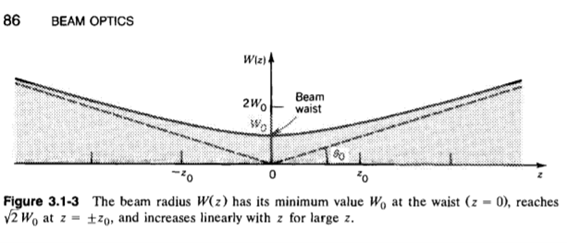
\includegraphics{beam_optics}[scale=1]
	\smallcaption{Fonte: SALEH, Bahaa E. A.; TEICH, Malvin Carl. Fundamentals of Photonics. 1.ed. Wiley-Interscience, 1991.}
	\smallcaption{Legenda: O raio do feixe $W_{(z)}$ tem seu valor mínimo no ponto eixo ($z = 0$), ele atinge $\sqrt{2} W_0$ quando $z=\pm z$, e aumenta linearmente com $z$ para valores de $z$ elevado.}
\end{figure}

\begin{equation}
\label{eq:raio_curvatura}
R_{(z)} = z \left [ 1 + \left( \frac{z}{z_0} \right ) ^2 \right ]
\end{equation}

\begin{equation}
\label{eq:fase_gouy}
\xi_{(z)} = tan^-1 \left( \frac{z}{z_0} \right )
\end{equation}

\begin{equation}
\label{eq:potencia_curvatura}
P=\frac{1}{2} I_0 \left( \pi W_0^2 \right )
\end{equation}

\begin{equation}
\label{eq:intensidade_eixo}
I_0 = \frac{E_0^2}{2 \eta}
\end{equation}

\begin{equation}
\label{eq:impedancia_meio}
\eta = \eta_0 \approx 377 \Omega
\end{equation}

Sendo o Raio de curvatura representado na equação \eqref{eq:raio_curvatura}, Fase de \emph{Gouy} representado na equação \eqref{eq:fase_gouy}, potência representado na equação \eqref{eq:potencia_curvatura} de acordo com e intensidade do eixo representado na equação \eqref{eq:intensidade_eixo}, sendo $\eta$ a impedância característica do meio, para o espaço livre (vide equação \eqref{eq:impedancia_meio}). Feixes ópticos são usualmente caracterizados pela potência $P$, então é útil escrever $I_0$ em temos de $P$ , equação \eqref{eq:i_p} [11].

\begin{equation}
\label{eq:i_p}
\eta = \eta_0 \approx 377 \Omega
\end{equation}

\subsubsection{Ângulo de divergência}

Longe do centro do feixe, o raio aumenta linearmente com $z$, definido um cone com meio ângulo \ang{80}, Figura \ref{fig:angulo_divergencia}, cerca de 86\% da potência do feixe é confinada dentro deste cone, sendo $\theta$ ângulo de divergência teta zero do feixe.

\begin{equation}
\label{eq:angulo_divergencia}
\theta_0 = \frac{2}{\pi} \frac{\lambda}{2 W_0}
\end{equation}

\begin{figure}[ht!]
	\centering
	\caption{Ângulo de divergência}
	\label{fig:angulo_divergencia}
	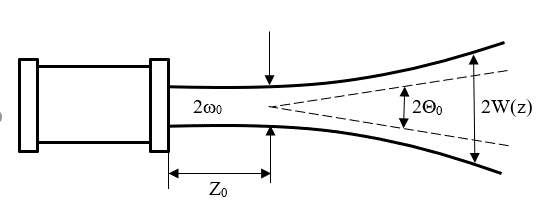
\includegraphics{angulo_divergencia}[scale=1]
	\smallcaption{Fonte: SALEH, Bahaa E. A.; TEICH, Malvin Carl. Fundamentals of Photonics. 1.ed. Wiley-Interscience, 1991.}
\end{figure}

\subsubsection{Profundidade de foco}

A profundidade de foco $Z_0$, é dada pela equação \ref{eq:prof_foco}, onde $\lambda$ é o comprimento de onda e $W_0$ é o raio do feixe na saída.

\begin{equation}
\label{eq:prof_foco}
2z_{0}=\frac{1 \pi W_0^2}{\lambda}
\end{equation}

\subsection{Segurança}

A colimação do feixe é o que difere a radiação do laser em relação aos outros tipos conhecidos de radiação, o comprimento de onda é o fator determinante para que o laser possa ser caracterizado como prejudicial. [12]

Na Figura \ref{espectro}, a parte amarela compreende o intervalo de comprimento de onda da atuação do laser.

\begin{figure}[ht!]
	\centering
	\caption{Intervalo do Espectro Eletromagnético onde o Laser atua}
	\label{fig:espectro}
	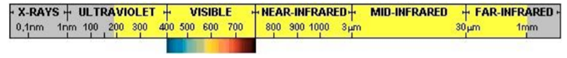
\includegraphics{espectro}[scale=1]
	\smallcaption{Fonte: Laser Institute of America, Laser Safety Information Bulletin, May 24, 2002.}
\end{figure}

Carroll [13] afirma que, em certas partes do corpo, tais como o globo ocular e os testículos, a conexão térmica com os tecidos circundantes é mínima e o fornecimento de sangue é inadequado para conduzir a energia desenvolvida pela exposição local ao laser. Quando estes órgãos estão expostos a tal tipo de radiação, podem produzir-se graves danos nos tecidos profundos dentro dos mesmos, onde há um grave risco de que causem cegueira ou esterilidade.

A periculosidade dos lasers infravermelhos se dá, principalmente, pelo fato da radiação invisível impossibilitar a resposta protetora de aversão ao brilho do corpo (``reflexo de piscar''), podendo causar danos imediatos na visão. Os demais efeitos biológicos da radiação podem ser consultados na Figura \ref{radiacao}.

\begin{figure}[ht!]
	\centering
	\caption{Efeitos biológicos da Radiação Laser}
	\label{fig:radiacao}
	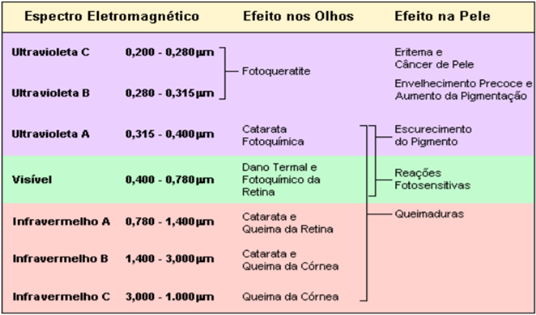
\includegraphics{radiacao}[scale=1]
	\smallcaption{Fonte: Laser Institute of America, Laser Safety Information Bulletin, May 24, 2002.}
\end{figure}

A maioria dos danos provocados pela radiação laser se deve ao aquecimento dos tecidos que a absorvem. Os lasers visíveis são particularmente perigosos, pois o olho humano focaliza o feixe na retina e esta pode sofrer queimaduras. A densidade de potência do ponto laser focalizado na retina é cerca de 100.000 vezes a densidade de potência incidente na córnea. Assim, embora seja relativamente seguro expor a pele a lasers visíveis de baixa potência, é sempre perigoso observar o feixe diretamente. [13]

Para realizar a avaliação dos riscos da exposição da radiação do laser, deve-se levar em conta as seguintes características:

\begin{itemize}
	\item Comprimento de onda;
	\item Potência;
	\item Duração e taxa de repetição;
	\item Diâmetro do feixe;
	\item Divergência.
\end{itemize}

\subsubsection{MPE}

A MPE (\emph{Maximum Permissible Exposure}) mede os níveis máximos permitidos de exposição levando em consideração a maior potência ou densidade de energia (\mbox{$W/cm^2$} ou \mbox{$J/cm^2$}) de uma fonte de luz que possa ser considerada segura. Essa medida é feita na córnea do olho humano ou pele, considerando o comprimento de onda, coerência temporal e coerência espacial. Na Tabela \ref{tab:mpe} pode-se observar o tempo máximo permitido de exposição em relação a alguns comprimentos de onda.

\begin{table}[ht!]
	\caption{Máxima exposição permitida}
	\label{tab:mpe}
	\begin{tabular}{c|c|c|c|c|c}
		\hline
		\multirow{2}{*}{\emph{Laser type}} & Wavelenght & MPE level (\mbox{$W/cm^2$})\\
		\cline{2-6}
		& (\mbox{$\mu$}) & 0.25 sec & 10 sec & 600 sec & 30,000 sec\\
		\hline
		
	\end{tabular}
	\smallcaption{Fonte: Adaptado de RIBEIRO, Martha Simões. INTERAÇÃO DA RADIAÇÃO LASER LINEARMENTE POLARIZADA DE BAIXA INTENSIDADE COM TECIDOS VIVOS: EFEITOS NA ACELERAÇÃO DE CICATRIZAÇÃO TISSULAR EM LESÕES DE PELE. 2000. 200 f. TCC}
\end{table}
\include{./cap/revisao_bibliografica/cap_subcap_pvcell}
\section{\emph{Wireless Power Transmission}}

Como o próprio nome já induz, essa tecnologia faz referência a uma forma eficiente de transferir energia elétrica sem o uso de qualquer substância ou fio. O intuito dela é ser usada em locais inacessíveis ou inconvenientes para utilização de outros meios físicos. Dentro dessa tecnologia, os meios mais comuns para fazer a transmissão de energia são o laser, ondas milimétricas ou micro-ondas.

Historicamente falando, essa tecnologia vem tentando ser aplicada desde 1897 quando Nikola Tesla deu início ao seu experimento com a \emph{``World Wireless''}, que mais tarde foi patenteada como \emph{``World Wireless System''}. O Primeiro eventual sucesso com a tecnologia \emph{Wireless Power Transmission} (WPT) só se deu em 1963 através da \emph{Raytheon Company}.

Quanto ao desenvolvimento do WPT, partindo do princípio de Lavoisier (1743-1794) “Na Natureza, nada se cria, nada se perde, tudo se transforma”, o primeiro passo é entender que a energia deve estar tratada de uma forma adequada para viajar pelo ar e, posteriormente, entender que isso nos levará ao desenvolvimento de um sistema para transmissão e recepção compatíveis para essa energia.

Com foco maior no nosso projeto, dentro dessa tecnologia, optamos por trabalhar com o modelo LPT, ou seja, uma transmissão via laser, que é um dos meios de transmissão direta, onde é necessário possuir visada entre o transmissor e receptor, o que limitará a distância de aplicação, mas não a eficiência. Iremos discutir a frente o desenvolvimento desse modelo.

\subsection{DLC - \emph{Distributed Laser Charging}}

O que diferencia o módulo DLC com os outros tipos de carregadores LPT é o sistema retrorrefletor que possibilita a segurança na transmissão de energia.

Utilizado em sinais de trânsito, bicicleta e automóveis, os retrorrefletores são “[...]sistemas ópticos que possuem a notável propriedade de, recebendo um raio luminoso, fazer com que ele retorne em uma direção paralela à de incidência com um mínimo de deslocamento.” [22]. Portanto, seu princípio de funcionamento engloba a Lei de Reflexão e a Lei da Refração.

No espelho de tela plana, a luz refletida é paralela a sua luz incidente somente quando o ângulo de incidência for vertical em relação ao espelho. Porém, no dispositivo, há três espelhos dispostos que, perpendicularmente, formam o retrorrefletor independentemente do seu ângulo de incidência, como mostra a figura \ref{retroreflector_cubo}.

\begin{figure}[ht!]
	\centering
	\caption{Retrorrefletor}
	\label{fig:retroreflector_cubo}
	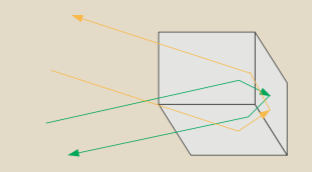
\includegraphics{retroreflector_cubo}[scale=1]
	\smallcaption{Fonte: ZHANG, FANGM KIU, WU, XIA, YANG: Distributed Laser Charging: A Wireless Power Transfer Appoach. IEEE Internet of Things journal, vol 5, no 5, pp 3853-3864, 2018. Disponível em: \url{https://ieeexplore.ieee.org/document/8398229/}. Acesso: 07 junho 2021.}
\end{figure}

DLC é uma tecnologia de \emph{Wireless Power Transfer} baseada em Lasers ressonantes e distribuídos. Os componentes óticos são divididos em duas partes, transmissor e receptor, respectivamente. 

A Figura 11 mostra o diagrama do sistema DLC. Um espelho retrorrefletor R1 com uma refletância de 100\% e um ganho médio estão presentes no transmissor. No receptor há um espelho R2 retrorrefletor com uma refletância parcial de 95\%. Os espelhos R1, R2 e o ganho médio formam a cavidade ressonante, onde os fótons são amplificados formando um laser ressonante de cavidade interna. Os fótons capazes de passar pelo espelho R2 formam o laser de cavidade externa. Este pode ser convertido em eletricidade através de uma célula fotovoltaica instalada atrás do espelho R2.

\begin{figure}[ht!]
	\centering
	\caption{Diagrama do sistema DLC}
	\label{fig:dlc}
	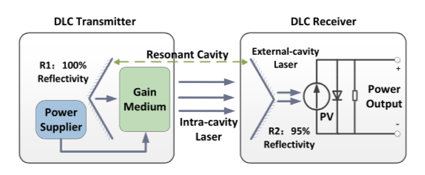
\includegraphics{dlc}[scale=1]
	\smallcaption{Fonte: ZHANG, FANGM KIU, WU, XIA, YANG: Distributed Laser Charging: A Wireless Power Transfer Appoach. IEEE Internet of Things journal, vol 5, no 5, pp 3853-3864, 2018. Disponível em: \url{https://ieeexplore.ieee.org/document/8398229/}. Acesso: 07 junho 2021.}
\end{figure}

No sistema DLC, fótons são amplificados sem a preocupação de seus ângulos de incidência, contanto que eles viajem dentro da linha de visão dos espelhos R1 e R2. Por isso, o laser de cavidade interna gerado pelo ressonador pode se auto alinhar sem um posicionamento ou rastreamento. Essa característica possibilita que usuários carreguem seus dispositivos sem um posicionamento cauteloso do mesmo. O Sistema DLC é intrinsecamente seguro, pois caso um objeto esteja bloqueando a linha de visão do laser de cavidade interna, o objeto pode parar o laser imediatamente, cancelando a ressonância. Essas características oferecem ao sistema DLC a capacidade de carregar dispositivos a longa distância.



\subsection{Dispositivos LPT disponíveis}

\subsubsection{PowerLight Technologies}

A \emph{PowerLight Technologies} é uma empresa americana de engenharia de transmissão de energia LPT que surgiu em 2006 com o nome de \emph{LaserMotive} para concorrer na \emph{Power Beam Challenge}, que faz parte da \emph{Centennial Challenges da NASA}. Após vencer o concurso de 2009, a empresa foca no desenvolvimento da tecnologia para alimentar VANTs (Veículo Aéreo Não Tripulado) e atua em parceria com a NASA para criar uma arquitetura que permite utilizar lasers para o lançamento de foguetes e satélites. [23].

\subparagraph{PowerLight Free-Space Power Beaming}

Em junho de 2012, a \emph{LaserMotive} conseguiu alimentar um \emph{Stalker Unmanned Aerial System} (UAS) da \emph{Lockheed Martin} por mais de 48 horas, sendo considerado um recorde na época [23].

\subsubsection{PTROL (Power Transmitted Over Laser) Project}

Em maio de 2019, a \emph{PowerLight} transmitiu 400 watts via laser a uma distância de 325 metros. O receptor converte a energia do laser em DC passando por um inversor que alimenta luzes, laptops e uma cafeteira.

As células fotovoltaicas no receptor foram modificadas para conseguir uma melhor resposta em um comprimento de onda e, também, no equipamento constava um sistema de segurança que interrompia a transmissão em qualquer obstáculo colocado entre o emissor e o receptor. [24]
\chapter{Desenvolvimento}

A metodologia será baseada no método \emph{Scrum, ``método ágil utilizado para a gestão e desenvolvimento de projetos que têm um curto prazo de entrega.''}.[25] Este método foi aplicado ao coletar os pontos positivos e negativos do grupo e definir os papeis de cada colaborador, considerando o nível de complexidade do projeto e o tempo disponível para sua elaboração.

As etapas do desenvolvimento do projeto descritas na Figura \ref{fig:etapas_dev} apresentam os parâmetros iniciais, escolha dos materiais e simulação. 

\begin{figure}[ht!]
\centering
\caption{Etapas de desenvolvimento}
\label{fig:etapas_dev}
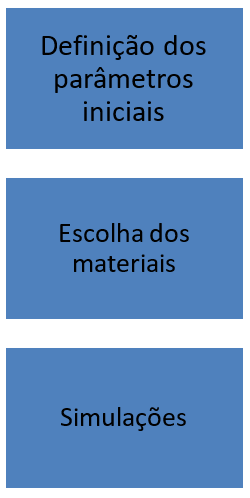
\includegraphics{etapas_dev}
\smallcaption{Fonte: Autor}
\end{figure}

\section{Parâmetros iniciais de projeto}

Os parâmetros iniciais de projeto foram determinados a partir das referências coletadas em artigos científicos e produtos disponíveis no mercado.

\begin{itemize}
	\item \mbox{$P_out$} = 5 W
	\item Distância de transmissão = 5 metros
	\item Eficiência > 50\%
\end{itemize}

\section{Sistema}

O sistema de transferência de energia a laser, foi elaborado baseando-se no sistema DLC [26].

No ganho médio os retrorrefletores permitem refletir fótons na mesma direção, mas com sentido aposto e com uma pequena defasagem. No retorno, os fótons passam pelo ganho médio onde o feixe é formado e é refletido novamente. O retrorrefletor no receptor permite que parte da energia do laser chegue na célula solar. Essa abordagem faz com que qualquer obstáculo entre o transmissor e o receptor, interrompa o laser, pois os fótons não voltam para formar o laser no ganho médio.

\subsection{Laser}

Para a seleção do laser, foram considerados os parâmetros:

\subsubsection{Possibilidade para transferir energia através da atmosfera}

A fim de maximizar a eficiência na transferência de energia, os lasers devem operar em uma faixa de energia em que as placas fotovoltaicas possam ser mais otimizadas. A janela na região entre 780 e 1100 nm é particularmente relevante para a tecnologia de transmissão de energia sem fio.

\subsubsection{Possibilidade para transferir a energia o maior tempo possível}

O feixe do laser deve ser brilhante o suficiente para garantir que a energia possa ser transferida em um longo intervalo de tempo. O fluxo $\Phi$ entregue ao receptor na faixa inclinada $L$ é dado pela equação.

\begin{equation}
\label{eq:gaussiano}
\Phi = \frac{R_{source} A_{source} \eta_{trans}}{L^2}
\end{equation}

Onde $R_{source}$ é a radiância (potência por unidade de área) da fonte do laser, uma constante que indica a qualidade do feixe e não pode ser alterada por ótica passiva; $A_{source}$ é a área total da fonte do feixe, $L$ é o alcance de transmissão e  $\eta_{trans}$ é a eficiência de transmissão através da atmosfera.

\subsubsection{Laser Diodo}

O laser diodo trabalhando no modo pulso, é a melhor opção para esse tipo de projeto, pois é o que apresenta melhor eficiência, confiabilidade e menor tamanho em relação aos outros tipos disponíveis no mercado [27].

A corrente injetada tem influência direta na eficiência de conversão que gira em torno de 50\% [27].

Para uma análise preliminar foram selecionados componentes que apresentam potência de saída maior que a requerida do projeto, Figura \ref{fig:modelo_1} e Figura \ref{fig:modelo_2}. Além disso, o tamanho também foi um dos pontos importantes para a seleção, sendo $I_{SE}$ é o índice \emph{Slope Efficiency}, \mbox{$P_{out_min}$} potência mínima de saída, \mbox{$E_{min}$} eficiência mínima e \mbox{$\lambda$} é o comprimento de onda, Tabela \ref{tab:comp_modelo}.

\begin{table}[ht!]
	\caption{Comparativo dos modelos selecionados}
	\label{tab:comp_modelo}
	\begin{tabular}{c|c|c|c|c|c}
		\hline
		\textbf{Laser} & \textbf{Modelo} & \textbf{\mbox{$P_{out_{min}}$} (W)} & \textbf{\mbox{$I_{SE}$} (W/A)} & \textbf{\mbox{$E_{min}$} (\%)} & \textbf{\mbox{$\lambda$} (nm)}\\
		\hline
		Laser 1 & RLS/LD-808NM-15W & 15 & 1,8 & 40 & 808\\
		\hline
		Laser 2 & K808DAECN-25.00W & 25 & 4 & 40 & 808\\
		\hline
		Laser 3 & RL915NM-10W & 10 & - & 40 & 915\\
		\hline
	\end{tabular}
	\smallcaption{Fonte: Adaptado de \url{http://pelicano.ipen.br/PosG30/TextoCompleto/Martha\%20Simoes\%20Ribeiro_D.pdf}. Acessado em: 22/05/2021}
\end{table}

\begin{figure}[ht!]
\centering
\caption{Optica do feixe}
\label{fig:modelo_1}
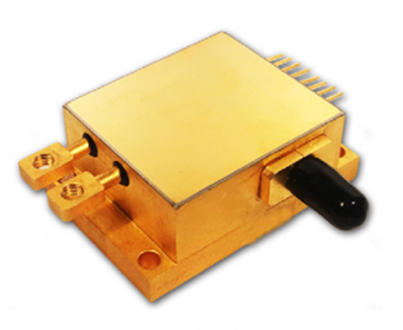
\includegraphics{modelo_1}
\smallcaption{Fonte: Laser Diode Source. Disponível em: \url{https://www.laserdiodesource.com/files/pdfs/laserdiodesource_com/4776/808nm_25W_Detachable_Fiber_Diode_Laser_BWT-1609445237.pdf}. Acesso em: 30 maio 2021.}
\end{figure}

\begin{figure}[ht!]
\centering
\caption{Optica do feixe}
\label{fig:modelo_2}
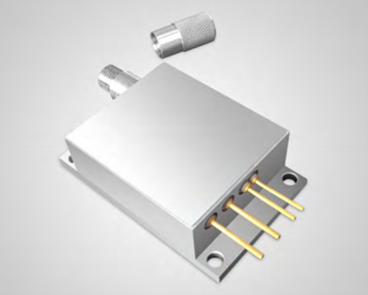
\includegraphics{modelo_2}
\smallcaption{Fonte: Laser Diode Source. Disponível em: \url{https://www.laserdiodesource.com/files/pdfs/laserdiodesource_com/4776/808nm_25W_Detachable_Fiber_Diode_Laser_BWT-1609445237.pdf}. Acesso em: 30 maio 2021.}
\end{figure}

\subsection{Painel Fotovoltaico}

Nas células fotovoltaicas, para gerar eletricidade, os fótons devem ter energia maior ou igual ao intervalo de banda do material. Uma vez que a energia de um fóton é proporcional à sua frequência, as células PV respondem a determinadas frequências de luz correspondentes ao intervalo de banda da célula energética.

Os principais fatores a serem considerados para que a potência possa ser efetivamente convertida em eletricidade são:

\begin{itemize}
	\item Potência do laser;
	\item Comprimento de onda;
	\item Temperatura;
	\item Material das células
\end{itemize}

As curvas de resposta espectral para alguns materiais de PV diferentes são ilustradas na Figura \ref{fig:resposta_espectral}.

\begin{figure}[ht!]
\centering
\caption{Resposta espectral}
\label{fig:resposta_espectral}
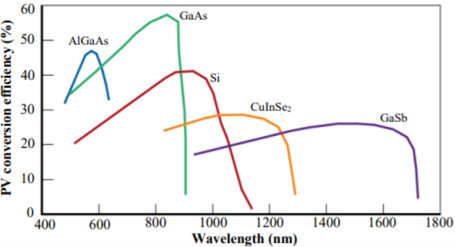
\includegraphics{resposta_espectral}
\smallcaption{Fonte: JIN, Ke; ZHOU, Weiyang. Wireless Laser Power Transmission: a review of recent progress. Ieee Transactions On Power Electronics, [s. l], v. 34, n. 4, p. 3842-3859, 05 jul. 2018. Disponível em: \url{https://ieeexplore.ieee.org/document/8404085}. Acesso em: 09 maio 2021.}
\end{figure}

Percebe-se que a célula fotovoltaica de Arseneto de Gálio (GaAs) apresenta uma melhor eficiência em relação ao comprimento de onda entre 800nm e 850nm. Porém, seu alto custo o torna inviável para utilização. Portanto, as células de Silício (Si) que apresentam uma melhor aplicação entre 850 nm e 1064 nm serão as utilizadas no projeto.
\include{./cap/simulacao/cap_simulacao}
\chapter{Conclusão}

Inicialmente o projeto foi idealizado com o objetivo de transferir energia utilizando um laser comercial. Entretanto, a necessidade de desenvolver um sistema de segurança impossibilitou a utilização de um laser convencional, o que aumentou consideravelmente a complexidade do trabalho sendo necessário o desenvolvimento de uma cavidade de ressonância externa para que o projeto pudesse ser concebido.

A dificuldade em realizar uma simulação relaciona-se com a necessidade do ganho médio, outro fator de grande dificuldade e que afetou o desenvolvimento da simulação do projeto foi a limitação dos softwares disponíveis no mercado. Além disso, essa nova forma de transmissão é muito recente e não há bibliografias especificas sobre o assunto disponíveis, apenas poucos artigos científicos.

Os resultados obtidos demonstram que o dispositivo apresenta uma baixa eficiência em decorrência de uma alta densidade de potência focada na célula da placa que afetou negativamente o desempenho da célula, entretanto pode-se confirmar que a perda em relação a distância é praticamente nula, o que mostra que raios lasers podem ser utilizados para transferir energia em grandes distâncias.

Apesar dos dados abaixo do esperado, o projeto continua sendo promissor, pois a ideia de transmitir energia de forma sem fio ainda é muito atrativa, principalmente em ambientes de smart home, lojas e shoppings. Além de haver espaço para o desenvolvimento de novas e melhores placas fotovoltaicas, aumentando a eficiência do conjunto.

\printbibliography
%\printindex
\end{document}